% Topic: relatório
% Created: 21-05-2025

\documentclass[]{abntex2}
\usepackage{pdfpages}
\usepackage[T1]{fontenc}
\usepackage[]{graphicx}
\usepackage[]{circuitikz}
\usepackage[]{hyperref}
\usepackage[]{amsmath}
\usepackage{booktabs}
\newtheorem{exemplo}{Exemplo}
\newcommand{\diff}{\ensuremath{\operatorname{d}\!}}
\usepackage{minted}
\usepackage[portuguese]{babel}

\begin{document}

\chapter{Desenvolvimento}
\section{Lâmpada}
Este projeto tem como objetivo o desenvolvimento de uma lâmpada inteligente com
controle de intensidade luminosa (\textit{dimmer}) e acionamento automático
baseado em sensores de luminosidade e presença. Para isso, foram utilizados um
microcontrolador ESP32C3 Super Mini, o sensor de luminosidade BH1750 e o sensor de presença por
radar LD2410C, além da integração com o sistema de automação residencial Home
Assistant OS (HAOS) via protocolo MQTT.

O desenvolvimento iniciou-se com uma prova de conceito, validando a comunicação
MQTT entre o microcontrolador e o \textit{addon} \textit{MQTT Broker} no HAOS.
A partir dessa etapa, foram realizadas as integrações dos sensores e a criação
de automações no Home Assistant.

\subsection{Conexão Wi-Fi}

A conexão Wi-Fi foi implementada com base no exemplo oficial disponível na
biblioteca Arduino
WiFi.\footnote{\url{https://github.com/arduino-libraries/WiFi/blob/master/examples/ConnectWithWPA/ConnectWithWPA.ino}}

O SSID e a senha da rede são armazenados em variáveis, e a função
\textit{WiFi.begin()} é utilizada para iniciar a conexão.

O status da conexão é exibido no monitor serial, permitindo a verificação do
sucesso da conexão e facilitando a depuração.

\begin{minted}{cpp}
const char* ssid = "HA AP";
const char* password = "12345678";

void connectToWiFi() {
  WiFi.begin(ssid, password);
  while (WiFi.status() != WL_CONNECTED) {
    delay(1000);
    Serial.println("Conectando ao Wi-Fi...");
  }
  Serial.println("Conectado ao Wi-Fi");
}
\end{minted}
\clearpage


\subsection{Conexão ao MQTT}

A conexão ao \textit{MQTT Broker} do HAOS foi desenvolvida com base no exemplo
oficial da biblioteca
PubSubClient.\footnote{\url{https://github.com/knolleary/pubsubclient/blob/master/examples/mqtt_basic/mqtt_basic.ino}}

O endereço IPv4 do HAOS, bem como o nome de usuário e a senha de um usuário
secundário, são armazenados em variáveis. A função \textit{client.setServer()}
é utilizada para definir o endereço IP e a porta do broker MQTT. A seguir, a
função \textit{client.setCallback()} registra o método que será executado
sempre que uma mensagem for recebida. A conexão é então estabelecida por meio
da função \textit{client.connect()}, que recebe como parâmetros o identificador
do cliente (no caso, o ESP) e as credenciais. O status da conexão é exibido no
monitor serial, auxiliando na depuração e no monitoramento da comunicação
MQTT.Após a conexão bem-sucedida, o ESP se inscreve nos tópicos de interesse
utilizando a função \textit{client.subscribe()}.

\begin{minted}{cpp}
const char* mqtt_server = "192.168.88.253";
const char* mqtt_user = "mosquito";
const char* mqtt_password = "12345";

WiFiClient espClient;
PubSubClient client(espClient);

void setupMQTT() {
  client.setServer(mqtt_server, 1883);
  client.setCallback(callback);

  while (!client.connected()) {
    Serial.println("Conectando ao MQTT...");
    if (client.connect("ESP32Client", mqtt_user, mqtt_password)) {
      Serial.println("Conectado ao MQTT");
      client.subscribe("topico/teste");
    } else {
      Serial.print("Falha, rc=");
      Serial.print(client.state());
      delay(5000);
    }
  }
}

void mqttLoop() {
  client.loop();
}
\end{minted}
\clearpage
\subsection{\textit{Callback} MQTT}

A função \textit{callback}, mencionada anteriormente, tem a função de processar
as mensagens recebidas nos tópicos em que o ESP está inscrito.

O conteúdo da mensagem, inicialmente recebido como um vetor de bytes, é
convertido para uma string, armazenado na variável \textit{message} e, em
seguida, exibido no monitor serial.

\begin{minted}{cpp}
void callback(char* topic, byte* payload, unsigned int length){
	String message = "";
	for (unsigned int i = 0; i < length; i++) {
		message += (char)payload[i];
	}

	Serial.print("Mensagem recebida [");
	Serial.print(topic);
	Serial.print("]: ");
	Serial.println(message);
}
\end{minted}

A comunicação MQTT foi testada pelo menu do add-on Mosquitto MQTT, publicando
mensagens nos tópicos e verificando a recepção no monitor serial.

\subsection{Teste dos Sensores}
Com a conexão Wi-Fi e o protocolo de comunicação MQTT funcionando corretamente,
prosseguiu-se com a implementação da leitura dos sensores no microcontrolador,
utilizando como base os exemplos disponibilizados nas bibliotecas dos
respectivos sensores.

\subsubsection{Sensor BH1750}

O código para leitura do sensor de luminosidade BH1750 foi desenvolvido com base no exemplo
oficial da biblioteca do sensor.
\footnote{\url{https://github.com/claws/BH1750/blob/master/examples/BH1750test/BH1750test.ino}}


Foi definido um tópico MQTT específico para o envio dos dados de luminosidade,
além de uma variável que controla o intervalo de leitura. A comunicação I2C é
inicializada com
\textit{Wire.begin()}, e o sensor é configurado com
\textit{lightMeter.begin()}.
Em cada intervalo de leitura, o valor de luminosidade em lux é obtido através
da função \textit{lightMeter.readLightLevel()}. Este valor, do tipo
\textit{float}, é convertido em \texttt{string} utilizando a função
\textit{dtostrf()}, e então publicado no tópico MQTT correspondente por meio de
\textit{client.publish()}.
\clearpage
\begin{minted}{cpp}
BH1750 lightMeter;
const char* topic_lux = "interruptor/lux";
uint32_t lastLuxReading = 0;

void initLuxSensor() {
  Wire.begin(2, 1);
  lightMeter.begin();
}

void readAndPublishLux() {
  if (millis() - lastLuxReading > 5000) {
    lastLuxReading = millis();
    float lux = lightMeter.readLightLevel();
    char luxStr[8];
    dtostrf(lux, 1, 2, luxStr);
    client.publish(topic_lux, luxStr);
  }
}
\end{minted}

\subsubsection{Sensor de Radar LD2410}

O código para integração do sensor de radar LD2410 foi desenvolvido com base no
exemplo oficial da biblioteca do sensor.
\footnote{\url{https://github.com/ncmreynolds/ld2410/blob/main/examples/basicSensor/basicSensor.ino}}

Inicialmente, define-se os pinos RX e TX utilizados na comunicação serial com o
radar, além da porta serial secundária (\textit{Serial1}). A função
\textit{initRadar()} realiza a inicialização da comunicação serial com o radar e
verifica se a conexão foi bem-sucedida. A função \textit{readAndPublishRadar()}
é executada periodicamente e realiza a leitura dos dados do sensor. Quando é
detectada uma mudança no estado de presença (presença detectada ou não
detectada), essa informação é publicada em um tópico MQTT específico. Quando a
presença é detectada, além do estado, também são coletadas e publicadas as
informações de distância e intensidade (energia) dos alvos, tanto estáticos
quanto em movimento, em seus respectivos tópicos MQTT.
\clearpage
\begin{minted}{cpp}
#define MONITOR_SERIAL Serial
#define RADAR_SERIAL Serial1
#define RADAR_RX_PIN 20
#define RADAR_TX_PIN 21
ld2410 radar;
uint32_t lastReading = 0;
bool presenceState = false;
void initRadar() {
  RADAR_SERIAL.begin(256000, SERIAL_8N1, RADAR_RX_PIN, RADAR_TX_PIN);
  if (radar.begin(RADAR_SERIAL)) {
    MONITOR_SERIAL.println(F("OK"));
  } else {
    MONITOR_SERIAL.println(F("NÃO CONECTADO"));
  }
}
void readAndPublishRadar() {
  if (millis() - lastReading > 1000) {
    lastReading = millis();
    radar.read();
    bool presenceDetected = radar.presenceDetected();
    if (presenceDetected && !presenceState) {
      client.publish("interruptor/radar", "Presença Detectada");
      presenceState = true;
    }
    else if (!presenceDetected && presenceState) {
      client.publish("interruptor/radar", "Presença Não Detectada");
      presenceState = false;
    }
    if (presenceDetected) {
      if (radar.stationaryTargetDetected()) {
        char distStr[8], energyStr[8];
        itoa(radar.stationaryTargetDistance(), distStr, 10);
        itoa(radar.stationaryTargetEnergy(), energyStr, 10);
        client.publish("interruptor/radar/estacionario/distancia", distStr);
        client.publish("interruptor/radar/estacionario/energia", energyStr);
      }
      if (radar.movingTargetDetected()) {
        char distStr[8], energyStr[8];
        itoa(radar.movingTargetDistance(), distStr, 10);
        itoa(radar.movingTargetEnergy(), energyStr, 10);
        client.publish("interruptor/radar/movendo/distancia", distStr);
        client.publish("interruptor/radar/movendo/energia", energyStr);
      }
    }
  }
}
\end{minted}

\subsection{Juntando todas as funções}
Com a estrutura modular do código finalizada e todas as funções devidamente
declaradas nos arquivos de cabeçalho (\textit{.h}) e implementadas nos arquivos
fonte (\textit{.cpp}) foi desenvolvido o código principal, responsável por
realizar a chamada das funções, utilizando o ambiente Arduino IDE.
\begin{minted}{cpp}
#include "wifi_manager.h"
#include "mqtt_manager.h"
#include "radar_sensor.h"
#include "lux_sensor.h"

void setup() {
  Serial.begin(115200);
  connectToWiFi();
  setupMQTT();
  initLuxSensor();
  initRadar();
}

void loop() {
  mqttLoop();
  readAndPublishLux();
  readAndPublishRadar();
}
\end{minted}

\subsection{Recebendo os dados no HA}
Com o \textit{addon} Mosquitto MQTT instalado no Home Assistant (HA), as
entidades são adicionadas por meio da edição do arquivo
\textit{configuration.yaml}, onde os sensores são configurados conforme a
documentação oficial do Home Assistant.

 \subsubsection{Definindo os sensores em YAML.}
Sensores MQTT são definidos em uma estrutura YAML, na qual se atribuem um nome
amigável, um identificador único para a entidade no HA e o tópico MQTT que
fornece os dados do sensor.

Declara-se um sensor para cada tópico MQTT previamente configurado no ESP.

\begin{minted}{yaml}
mqtt:
  sensor:
    - name: "Lux"
      unique_id: sensor_lux
      state_topic: "interruptor/lux"
      device_class: illuminance
    - name: "Presença Estacionária Distância"
      unique_id: sensor_est_dis
      state_topic: "interruptor/radar/estacionario/distancia"
    - name: "Presença Estacionária Energia"
      unique_id: sensor_est_ene
      state_topic: "interruptor/radar/estacionario/energia"
    - name: "Presença Em Movimento Distância"
      unique_id: sensor_mov_dis
      state_topic: "interruptor/radar/movendo/distancia"
    - name: "Presença Em Movimento Energia"
      unique_id: sensor_mov_ene
      state_topic: "interruptor/radar/movendo/energia"
    - name: "Presença Detectada"
      unique_id: sensor_mov_pre
      state_topic: "interruptor/radar"
\end{minted}

Com os dados armazenados nas entidades, eles podem ser utilizados de diversas
formas no (HA). Para os propósitos deste projeto, o foco será na
criação de automações.

\subsection{Automações}
As automações no HA podem ser definidas diretamente no arquivo
\textit{automations.yaml} ou utilizando o editor de blocos visual disponível na
interface do HA.

\subsubsection{\textit{Switch} para a lâmpada}

Foi criada uma automação com o objetivo de ligar e desligar a lâmpada com base
no estado do sensor de presença. Para isso, é necessário configurar um
\textit{switch} MQTT, declarado no arquivo \textit{configuration.yaml}, da
seguinte forma:
\clearpage
\begin{minted}{yaml}
mqtt:
  switch:
    - name: "Lampada"
      unique_id: lampada
      state_topic: "interruptor/switch"
      command_topic: "interruptor/switch"
      payload_on: "1"
      payload_off: "0"
\end{minted}
Com essa configuração, é criada uma entidade do tipo \textit{switch} que
publica o valor \textit{"1"} no tópico \texttt{interruptor/switch} quando está
ligada, e \textit{"0"} quando está desligada.

Devido à natureza do MQTT, caso o estado seja alterado por outro dispositivo ou
por outro processo dentro do HA, a entidade será atualizada automaticamente
para refletir essa mudança.

Com a entidade devidamente configurada, foram criadas duas automações: uma para
ligar o \textit{switch} quando for detectada presença, e outra para desligá-lo
após um tempo arbitrário sem detecção de presença.

\begin{minted}{yaml}
id: '1743357707824'
  alias: Detector de Presença (Ligar)
  description: Liga a lampada se presença detectada
  triggers:
  - entity_id:
    - sensor.presenca_detectada
    from: Presença Não Detectada
    to: Precença Detectada
    trigger: state
  conditions: []
  actions:
  - action: switch.turn_on
    metadata: {}
    data: {}
    target:
      entity_id: switch.lampada
  mode: single
- id: '1745710625710'
  alias: Sensor de Presença (Desligar)
  description: Desliga a lampada se presença não detectada
  triggers:
  - entity_id:
    - sensor.presenca_detectada
    to: Presença Não Detectada
    trigger: state
    from: Presença Detectada
    for:
      hours: 0
      minutes: 3
      seconds: 0
  conditions: []
  actions:
  - action: switch.turn_off
    metadata: {}
    data: {}
    target:
      entity_id: switch.lampada
  mode: single
\end{minted}
\clearpage

Ao inscrever o ESP neste tópico, torna-se possível monitorar e reagir às
mudanças de estado publicadas.

Na função \textit{setupMQTT()}

\begin{minted}{cpp}
void setupMQTT() {
client.subscribe("interruptor/switch");
}
\end{minted}

Para controlar a lâmpada por meio de um relé, é utilizada uma estrutura
condicional \textit{if} dentro da função \texttt{callback()}.
Nessa função, a comparação entre a variável \textit{topic} e o tópico definido
no HA é feita utilizando a função \textit{strcmp()}.
O valor da mensagem (\textit{message}) é então verificado, e, com base nesse
valor, a função \textit{digitalWrite()} altera o estado lógico do pino
conectado ao relé.

Na função \textit{callback()}
\begin{minted}{cpp}
const int pinoRELE = 0;
void callback(char* topic, byte* payload, unsigned int length) {
	String message = "";
	for (unsigned int i = 0; i < length; i++) {
		message += (char)payload[i];
	}
	if (strcmp(topic, "interruptor/switch") == 0) {
		if (message == "1") {
			digitalWrite(pinoRELE, HIGH);
		} else if (message == "0") {
			digitalWrite(pinoRELE, LOW);
		}
	}
}
\end{minted}
\subsubsection{Controle de brilho da lâmpada}
Utilizando os valores lidos e publicados no tópico do sensor de luminosidade, é
possível automatizar o controle do brilho da lâmpada.

Foi adicionada uma entidade do tipo \textit{number} no arquivo
\textit{configuration.yaml}, responsável por publicar e receber dados no tópico
específico.
\begin{minted}{yaml}
mqtt:
  number:
    - name: "Brilho"
      unique_id: mqtt_slider_Brilho
      state_topic: "lampada/brilho"
      command_topic: "lampada/brilho"
      min: 0
      max: 100
      step: 1
      retain: false
      unit_of_measurement: "%"
\end{minted}
Foi criada uma automação usando a fórmula sugerida nos fórums do HA
\footnote{\url{https://community.home-assistant.io/t/dim-lights-as-lumens-increases/182065/15}}
e usando como base o \textit{blueprint} \footnote{\url{https://community.home-assistant.io/t/smart-lux-dimmer-adjust-light-brightness-depending-on-light-sensor-value/403646}}
\[
	Brilho = (Declive \times  lux) + constante
\]
No arquivo \textit{automations.yaml} Onde são definidas as variáveis
\textit{maxB}, que representa o valor de lux no qual o brilho é configurado em
0 (correspondente à variável \textit{light\_value\_1}), e \texttt{minB}, que é o
valor de lux onde o brilho atinge 100\% (definido pela variável
\textit{light\_value\_2}).\[
slope= \frac{light1 - light2}{maxB - minB}
\]
e a constante pela formula:
\[
constant = light1 - (slope \times maxB)
\]


\begin{minted}{yaml}
- id: '1745186830191'
  alias: Dimmer
  description: Configura Brilho baseado em um valor alvo
  triggers:
  - entity_id: sensor.lux
    trigger: state
  conditions:
  - condition: numeric_state
    entity_id: sensor.lux
    above: 0
  actions:
  - target:
      entity_id: number.brilho
    data:
      value: "\n  0\n\n  {{ (( slope
        * states(light_sensor)|int ) + constant)|round }}\n\n"
    action: number.set_value
  variables:
    light_sensor: sensor.lux
    maxB: 400
    minB: 0
    light_value_1: 0
    light_value_2: 100
    light1: '{{ light_value_1 * 1 }}'
    light2: '{{ light_value_2 * 1 }}'
    slope: '{{ ( light1 - light2 ) / ( maxB - minB ) }}'
    constant: '{{ light1 - ( slope * maxB ) }}'
  mode: single
\end{minted}

O ESP também é inscrito neste tópico para receber os comandos de controle de
brilho.

Na função \textit{setupMQTT()}
\begin{minted}{cpp}
void setupMQTT() {
	client.subscribe("lampada/brilho");
}
\end{minted}

Na função \textit{setupPWM()}, são definidas as configurações do sinal PWM,
incluindo frequência, resolução e o pino utilizado.
A função \textit{ledcAttach()} do ESP é utilizada para vincular o pino
ao canal PWM com os parâmetros definidos.
Na funcão \textit{callback}, o valor recebido é limitado ao intervalo de 0 a 100 e, em seguida, convertido
proporcionalmente para o intervalo de 0 a 255, que representa o \textit{Duty
Cycle} do sinal PWM no ESP.
Por fim, a função \textit{ledcWrite()} ajusta o sinal PWM no pino, aplicando o
\textit{Duty Cycle} correspondente ao valor de brilho recebido no tópico
\textit{lampada/brilho}.

\begin{minted}{cpp}
const int pwmFreq = 20000;  // Frequência de 20kHz
const int pwmResolution = 8; // Resolução de 8 bits (0-255)
const int pinoPWM = 10;
void setupPWM() {
	ledcAttach(pinoPWM, pwmFreq, pwmResolution);
}
void callback(char* topic, byte* payload, unsigned int length) {
	if (strcmp(topic, "lampada/brilho") == 0) {
		int brilho = constrain(message.toInt(), 0, 100);
		int pwm = (255.0 / 100.0) * brilho;
		ledcWrite(pinoPWM, pwm);
	}
}
\end{minted}
Também é adicionada a função \textit{setupPWM} dentro da função
\textit{setup()} do arquivo principal.
\begin{minted}{cpp}
void setup(){
setupPWM();
}
\end{minted}



\subsection{Modificando uma lâmpada}
Lâmpadas de LED convencionais não permitem ajuste de brilho dinâmico da mesma
forma que lâmpadas de tecnologias anteriores.

Para possibilitar o ajuste de brilho em lâmpadas de LED modernas, que utilizam
circuitos integrados simples para controle de potência, adotou-se o princípio
demonstrado neste vídeo
\footnote{\url{https://www.youtube.com/watch?v=5HTa2jVi_rc}}, mas ao
Entretanto, em vez de alterar os resistores para reduzir a potência
da lâmpada, optou-se por utilizar um transistor que recebe o sinal PWM do ESP,
configurado anteriormente no lugar de um dos resistores, permitindo o
controle dinâmico do brilho.

\begin{figure}[h]
\centering
\begin{circuitikz}[american]
	\draw (0,0) node{RS1} to [R=$ 5 \Omega $] (0,2) -- (1, 2)
to [R=$ 501K \Omega $] (1,4)  to [led] (1,6) -- (1, 7) -- (4, 7) -- (4, 0) node[ground]{}
\draw (1,2) -- (2, 2) to [R=$ 10 \Omega $] (2,0) node{RS2}
;
\end{circuitikz}
\caption{Circuito original}
\end{figure}

\begin{figure}[h]
\centering
\begin{circuitikz}[american]
    \draw (0,0) node[]{RS1} to[short] (0,0.5);
    \draw (0,0.5) node[npn, anchor=E, xscale=1] (Q1) {};
    \node at (-0.3,1.1) {};

    \draw (Q1.C) -- (0,2) to[R=$5\,\Omega$] (0,4);

    \draw (0,4) -- (1,4)
    to[R=$501\,k\Omega$] (1,6)
    to[led] (1,8) -- (1,9) -- (4,9) -- (4,0) node[ground]{};

    \draw (1,4) -- (2,4) to[R=$10\,\Omega$] (2,0) node[]{RS2};

    \draw (Q1.B) -- ++(-1,0) to[R=$75\Omega$] ++(0,2) node[]{PWM};
\end{circuitikz}
\caption{Circuito modificado}
\end{figure}
\clearpage
Dessa forma, concluem-se todos os objetivos desta etapa do projeto: a lâmpada
pode ser ligada e desligada via relé controlado pelo Home Assistant, e seu
brilho pode ser ajustado dinamicamente através de um sinal PWM, também
controlado pelo Home Assistant. A montagem do projeto foi realizada conforme  a
esquemática apresentada.

\includepdf{\detokenize{~/Engenharia Elétrica/5 Semestre/Projeto Integrador/Trabalho/LampadaMqtt/output.pdf}}

\section{Climatização}
Este projeto tem como objetivo o desenvolvimento de um sistema de controle para
climatização, com acionamento automático por meio de um relé, baseado na
leitura de temperatura e em uma temperatura alvo definida.
Para a implementação, foram utilizados um microcontrolador ESP32-C3 Super Mini,
o sensor de temperatura e umidade AHT10, além da comunicação com o Home
Assistant (HA) através do protocolo MQTT.

Grande parte dos módulos de código desenvolvidos anteriormente foram
reutilizados, com uma alteração necessária:
o identificador do cliente MQTT precisa ser diferente do utilizado no outro
dispositivo, a fim de evitar conflitos na comunicação.

\begin{minted}{cpp}

void setupMQTT() {
    if (client.connect("ESP32Client2", mqtt_user, mqtt_password)) {
}
\end{minted}
\subsection{Sensor AHT10}
O código para leitura do sensor de temperatura e umidade AHT10 foi
desenvolvido com base no exemplo oficial da biblioteca do sensor. \footnote{\url{https://github.com/adafruit/Adafruit_AHTX0/blob/master/examples/adafruit_aht_test/adafruit_aht_test.ino}}
A função \textit{readAndPublishTemp()} é executada periodicamente
realizando a leitura dos dados do sensor.
Estes valores, do tipo float, são convertidos em strings utilizando a
função \textit{dtostrf()}, e então publicados nos tópicos MQTT correspondentes por meio de \textit{client.publish()}.

\begin{minted}{cpp}
Adafruit_AHT10 aht;

void init_Temp() {

  if (! aht.begin()) {
    Serial.println("Could not find AHT10? Check wiring");
    while (1) delay(10);
  }
  Serial.println("AHT10 found");
}

void readAndPublishTemp() {
	sensors_event_t humidity, temp;
	aht.getEvent(&humidity, &temp);
	char tempStr[8], humiStr[8];
    dtostrf(temp.temperature, 1, 2, tempStr);
    dtostrf(humidity.relative_humidity, 1, 2, humiStr);
	client.publish("sensor/humi", humiStr);
	client.publish("sensor/temp", tempStr);

  delay(500);
}
\end{minted}

\subsection{Juntando as funções}
Com a estrutura modular do código finalizada e todas as funções devidamente
declaradas nos arquivos de cabeçalho (.h) e implementadas nos arquivos fonte
(.cpp) foi desenvolvido o código principal, responsável por realizar a chamada
das funções, utilizando o ambiente Arduino IDE.

\begin{minted}{cpp}
#include "wifi_manager.h"
#include "mqtt_manager.h"
#include "temperature_sensor.h"


void setup() {
  Serial.begin(115200);
  connectToWiFi();
  setupMQTT();
  init_Temp();
}

void loop() {
  mqttLoop();
  readAndPublishTemp();
}
\end{minted}

\subsection{Recebendo os dados no HA}
\subsubsection{Definido o sensor em YAML}
\begin{minted}{yaml}
  sensor:
    - name: "Temperatura"
      unique_id: sensor_temp
      state_topic: "sensor/temp"
    - name: "humidade"
      unique_id: sensor_humi
      state_topic: "sensor/humi"
\end{minted}

\subsubsection{Automação}
Para a definição da temperatura alvo foi necessário criar uma entidade do tipo \textit{number}, como não é necessária transmissão MQTT desse valor podemos criar a entidade na GUI do HA.
\clearpage
\begin{figure}[h]
\centering
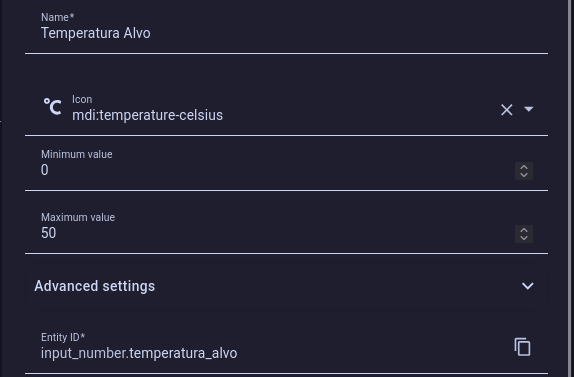
\includegraphics[width=0.9\textwidth]{\detokenize{~/Engenharia Elétrica/5 Semestre/Projeto Integrador/Trabalho/relatório/Temperatura.png}}
\caption{Criação de entidade \textit{number} no HA}
\end{figure}
\clearpage
E também é necessário criar outro \textit{switch} MQTT no arquivo \textit{configuration.yaml} com um tópico MQTT.
\begin{minted}{yaml}
mqtt:
  switch:
    - name: "Climatização"
      unique_id: cont_climat
      state_topic: "climatização/rele"
      command_topic: "climatização/rele"
      payload_on: "1"
      payload_off: "0"
\end{minted}


Agora a automação pode ser criada, de maneira a ligar e desligar o relé para atingir a temperatura alvo
\begin{minted}{yaml}
- id: '1747447570318'
  alias: Climatização
  description: ''
  triggers:
  - trigger: state
    entity_id:
    - sensor.temperatura
    - input_number.temperatura_alvo
  conditions: []
  actions:
  - choose:
    - conditions:
      - condition: numeric_state
        entity_id: sensor.temperatura
        above: input_number.temperatura_alvo
        below: 51
      sequence:
      - action: switch.turn_on
        metadata: {}
        data: {}
        target:
          entity_id: switch.climatizacao
    - conditions:
      - condition: numeric_state
        entity_id: sensor.temperatura
        below: input_number.temperatura_alvo
        above: '0'
      sequence:
      - action: switch.turn_off
        metadata: {}
        data: {}
        target:
          entity_id: switch.climatizacao
  mode: single
\end{minted}

O ESP é inscrito neste tópico.
\begin{minted}{cpp}
void setupMQTT() {
client.subscribe("climatização/rele");
}
\end{minted}

Para controlar o relé, é utilizada uma estrutura
condicional \textit{if} dentro da função \texttt{callback()}.
Nessa função, a comparação entre a variável \textit{topic} e o tópico definido
no HA é feita utilizando a função \textit{strcmp()}.
O valor da mensagem (\textit{message}) é então verificado, e, com base nesse
valor, a função \textit{digitalWrite()} altera o estado lógico do pino
conectado ao relé.

Na função \textit{callback()}
\begin{minted}{cpp}
const int pinoRELE = 0;
void callback(char* topic, byte* payload, unsigned int length) {
	String message = "";
	for (unsigned int i = 0; i < length; i++) {
		message += (char)payload[i];
	if (strcmp(topic, "climatização/rele") == 0) {
		if (message == "1") {
			digitalWrite(pinoRELE, HIGH);
		} else if (message == "0") {
			digitalWrite(pinoRELE, LOW);
		}
	}
}
\end{minted}

Dessa forma, concluem-se todos os objetivos desta etapa do projeto: o relé é
controlado pelo Home Assistant, com base em uma temperatura alvo definida pelo
usuário. A montagem do projeto foi realizada conforme  a esquemática apresentada.
\clearpage
\includepdf{\detokenize{~/Engenharia Elétrica/5 Semestre/Projeto Integrador/Trabalho/ClimatizaçãoMqtt/output.pdf}}

\end{document}
